% BTP presentation: Constructing Code Property Graphs from Clang IR
% Compile with: pdflatex CPG.tex   (run twice), or upload to Overleaf.
\documentclass[aspectratio=169,10pt]{beamer}

\usetheme{Madrid}
\usecolortheme{default}

% Custom IITG Blue/Teal Palette
\definecolor{IITGBlue}{RGB}{0, 82, 147}
\definecolor{IITGAccent}{RGB}{0, 128, 128}
\definecolor{hl}{RGB}{200, 90, 20}      % highlight colour for diagrams
\definecolor{okgreen}{RGB}{0, 130, 60}
\definecolor{badred}{RGB}{180, 30, 30}
\definecolor{callblue}{RGB}{40, 80, 200}
\definecolor{flowgreen}{RGB}{40, 130, 60}
\setbeamercolor{palette primary}{bg=IITGBlue, fg=white}
\setbeamercolor{palette secondary}{bg=IITGAccent, fg=white}
\setbeamercolor{palette tertiary}{bg=IITGBlue, fg=white}
\setbeamercolor{structure}{fg=IITGBlue}
\setbeamertemplate{navigation symbols}{}
% Footer: only "slide / total" at the bottom right
\setbeamertemplate{footline}{%
  \hfill\usebeamercolor[fg]{structure}\scriptsize\insertframenumber\,/\,\inserttotalframenumber\hspace*{1em}\vspace*{0.6em}}
\setbeamertemplate{itemize items}[circle]

\usepackage[T1]{fontenc}
\usepackage{lmodern}
\usepackage{graphicx}
\usepackage{booktabs}
\usepackage{array}
\usepackage{tabularx}
\usepackage{pifont}
\usepackage{listings}
\usepackage{tikz}
\usetikzlibrary{arrows.meta,positioning,shapes.geometric,fit,backgrounds,calc}

\newcommand{\cmark}{\textcolor{okgreen}{\ding{51}}}
\newcommand{\xmark}{\textcolor{badred}{\ding{55}}}
\newcommand{\pmark}{\textcolor{hl}{$\sim$}}
\newcommand{\code}[1]{\texttt{#1}}

\lstset{
  basicstyle=\ttfamily\scriptsize,
  columns=fullflexible,
  keepspaces=true,
  showstringspaces=false,
  frame=single,
  rulecolor=\color{gray!50},
  backgroundcolor=\color{gray!6},
  xleftmargin=2pt,
  xrightmargin=2pt,
  aboveskip=2pt,
  belowskip=2pt,
  keywordstyle=\color{IITGBlue}\bfseries,
  commentstyle=\color{gray}\itshape,
}
\lstdefinelanguage{CIR}{
  morekeywords={cir.func,cir.alloca,cir.store,cir.load,cir.const,cir.cmp,
    cir.if,cir.scope,cir.return,cir.call,cir.add,cir.trap,cir.ternary,cir.yield},
  alsoletter={.},
  sensitive=true,
  morecomment=[l]{//},
}
\lstdefinelanguage{LLVMIR}{
  morekeywords={define,alloca,store,load,icmp,br,label,ret,select,ptr,i32,i1},
  sensitive=true,
  morecomment=[l]{;},
}
\lstdefinelanguage{Cypher}{
  morekeywords={MATCH,WHERE,RETURN,AND,ORDER,BY,LIMIT},
  sensitive=true,
  morecomment=[l]{//},
}

% Title & Institute Details
\title[CPGs from Clang IR]{Constructing Code Property Graphs from Clang IR\\for C and C++ Program Analysis}
\subtitle{B.Tech Project Presentation}
\author[Maheshwari, Agarwal]{Kartik Maheshwari \and Atharv Agarwal \\ \small Supervisor: Prof.~Bernard Nongpoh}
\institute[IIT Guwahati]{Department of Computer Science and Engineering \\ Indian Institute of Technology Guwahati}
\date{\today}

% Logo on Title Page (shown only if iitg_logo.png is present next to this file)
\IfFileExists{iitg_logo.png}{\titlegraphic{\includegraphics[height=1.6cm]{iitg_logo.png}}}{}

\begin{document}

% ----------------------------------------------------------------
\begin{frame}
  \titlepage
\end{frame}

% ----------------------------------------------------------------
\begin{frame}{Outline}
  \tableofcontents
\end{frame}

% ================================================================
\section{The Problem}
% ================================================================

% ----------------------------------------------------------------
\begin{frame}{Static Analysis of C/C++}
  \textbf{Static analysis}: reasoning about a program \textbf{without running it}

  \vspace{0.8em}
  \begin{columns}[T]
    \begin{column}{0.48\textwidth}
      \textbf{Typical questions}
      \begin{itemize}
        \item Who calls \code{parse()}, across all files?
        \item Which store does this load read?
        \item Is this function ever reachable?
        \item Which inputs reach this branch?
      \end{itemize}
    \end{column}
    \begin{column}{0.48\textwidth}
      \textbf{Why C/C++ is hard}
      \begin{itemize}
        \item Many translation units (TUs), linked later
        \item Overloads, templates, implicit conversions
        \item Side effects hidden behind pointers / references
        \item Same-named \code{static} symbols in different files
      \end{itemize}
    \end{column}
  \end{columns}

  \vspace{1.2em}
  \begin{block}{}
    \centering
    Needs three views: \textbf{call graph} \quad + \quad \textbf{control flow}
    \quad + \quad \textbf{data flow}
  \end{block}
\end{frame}

% ----------------------------------------------------------------
\begin{frame}{Problem Statement}
  \begin{alertblock}{Goal}
    A \textbf{general-purpose}, compiler-accurate, whole-program
    \textbf{Code Property Graph} for C/C++ that answers \textbf{queries}
    about a codebase
  \end{alertblock}

  \vspace{0.6em}
  \begin{columns}[T]
    \begin{column}{0.48\textwidth}
      \textbf{Requirements}
      \begin{itemize}
        \item \textbf{Compiler-accurate}: types, overloads, names
        \item \textbf{Whole program}: all TUs, \code{static} vs.\ \code{extern}
        \item \textbf{Multi-level}: functions, blocks, values
        \item \textbf{Queryable}: graph database + Cypher
      \end{itemize}
    \end{column}
    \begin{column}{0.48\textwidth}
      \textbf{Example uses}
      \begin{itemize}
        \item Code navigation (callers, callees, reachability)
        \item Data-flow tracing / slicing
        \item \textbf{AI agents} querying the graph instead of reading source
              \begin{itemize}
                \item e.g.\ test generation (case study)
              \end{itemize}
      \end{itemize}
    \end{column}
  \end{columns}
\end{frame}

% ================================================================
\section{ClangIR (CIR)}
% ================================================================

% ----------------------------------------------------------------
\begin{frame}{Where CIR Sits in the Compiler}
  \centering
  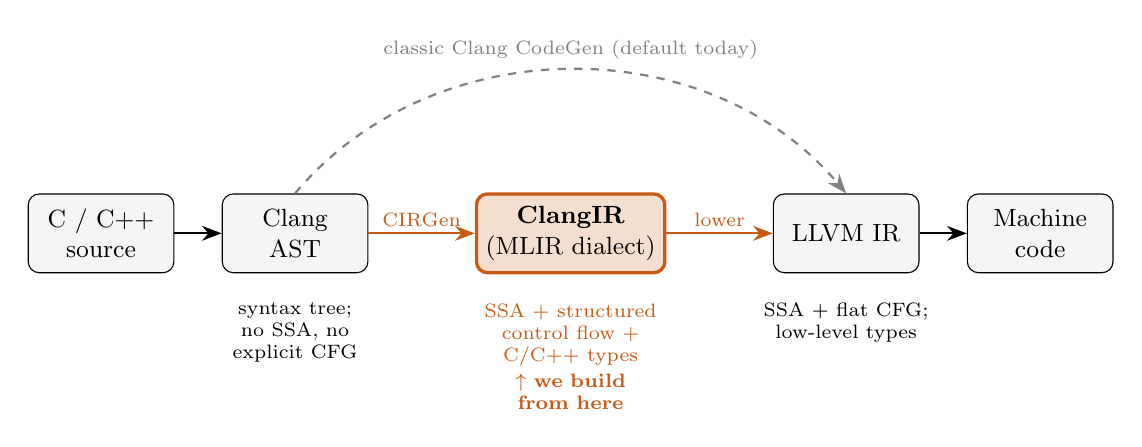
\begin{tikzpicture}[
      stage/.style={draw, rounded corners, minimum height=1.0cm, minimum width=1.85cm,
                    align=center, font=\small, fill=gray!8},
      ours/.style={stage, fill=hl!20, draw=hl, very thick},
      arr/.style={-{Stealth[length=2.5mm]}, thick},
      lab/.style={font=\scriptsize, above, inner sep=2pt}]
    \node[stage] (src) {C / C++\\source};
    \node[stage, right=0.6cm of src] (ast) {Clang\\AST};
    \node[ours, right=1.35cm of ast] (cir) {\textbf{ClangIR}\\(MLIR dialect)};
    \node[stage, right=1.35cm of cir] (llvm) {LLVM IR};
    \node[stage, right=0.6cm of llvm] (mc) {Machine\\code};
    \draw[arr] (src) -- (ast);
    \draw[arr, hl] (ast) -- node[lab]{CIRGen} (cir);
    \draw[arr, hl] (cir) -- node[lab]{lower} (llvm);
    \draw[arr] (llvm) -- (mc);
    \draw[arr, dashed, gray] (ast.north) to[out=50, in=130]
      node[above, font=\scriptsize]{classic Clang CodeGen (default today)} (llvm.north);
    \node[below=0.25cm of ast, font=\scriptsize, align=center, text width=2.3cm]
      {syntax tree;\\no SSA, no explicit CFG};
    \node[below=0.25cm of cir, font=\scriptsize, align=center, text width=2.8cm, text=hl]
      {SSA + structured\\control flow + C/C++ types\\[0.15em]
       \textbf{$\uparrow$ we build from here}};
    \node[below=0.25cm of llvm, font=\scriptsize, align=center, text width=2.3cm]
      {SSA + flat CFG;\\low-level types};
  \end{tikzpicture}

  \vspace{0.6em}
  \begin{itemize}
    \item MLIR-based IR in upstream LLVM, generated directly from the Clang AST
    \item \textbf{Structured control flow}: \code{cir.if}, \code{cir.for},
          \code{cir.while}, \code{cir.switch}, \code{cir.try}
    \item \textbf{Source types and locations} on every operation
    \item Already \textbf{SSA}: explicit def--use chains
  \end{itemize}
\end{frame}

% ----------------------------------------------------------------
\begin{frame}[fragile]{Same Function: CIR vs.\ LLVM IR}
  \lstset{moredelim=**[is][\color{hl}\bfseries]{|}{|}}
  \begin{columns}[T]
    \begin{column}{0.29\textwidth}
      \textbf{Source (C++)}
\begin{lstlisting}[language=C++]
struct Account {
  int id;
  int balance;
};

void deposit(Account &a,
             int amt) {
  a.balance += amt;
}
\end{lstlisting}
      \vspace{0.3em}
      \textbf{LLVM IR, \code{-O1}}
\begin{lstlisting}[language=LLVMIR]
%3 = getelementptr
       |i8, ptr %0, i64 4|
%4 = load i32, ptr %3
%5 = add nsw i32 %4, %1
store i32 %5, ptr %3
\end{lstlisting}
    \end{column}
    \begin{column}{0.37\textwidth}
      \textbf{ClangIR}
\begin{lstlisting}[language=CIR]
cir.func @_Z7depositR7Accounti(
    %arg0: |!cir.ptr<!rec_Account>|,
    %arg1: !s32i) {
  %0 = cir.alloca |"a"|
  %1 = cir.alloca |"amt"|
  ...
  %3 = cir.load %0
  %4 = cir.get_member %3[1]
         |{name = "balance"}|
  %5 = cir.load %4 : !s32i
  %6 = cir.add nsw %5, %2
  cir.store %6, %4
\end{lstlisting}
    \end{column}
    \begin{column}{0.31\textwidth}
      \textbf{LLVM IR, \code{-O0}}
\begin{lstlisting}[language=LLVMIR]
define void
  @_Z7depositR7Accounti(
    |ptr %0|, i32 %1) {
  %3 = alloca ptr
  %4 = alloca i32
  ...
  %6 = load ptr, ptr %3
  %7 = getelementptr
         %struct.Account,
         ptr %6, |i32 0, i32 1|
  %8 = load i32, ptr %7
  %9 = add nsw i32 %8, %5
  store i32 %9, ptr %7
\end{lstlisting}
    \end{column}
  \end{columns}

  \vspace{0.4em}
  \small
  \begin{itemize}
    \item LLVM IR: \code{Account\&} is just \code{ptr}; \code{balance} is index 1 (\code{-O0}) or byte offset 4 (\code{-O1})
    \item ClangIR: class type, variable names and field name kept
  \end{itemize}
\end{frame}

% ----------------------------------------------------------------
\begin{frame}{Why ClangIR, Not the AST or LLVM IR?}
  \begin{columns}[T]
    \begin{column}{0.48\textwidth}
      \textbf{Clang AST: drawbacks}
      \begin{itemize}
        \item Syntax tree, not an IR
        \item No explicit CFG
        \item No SSA values
        \item Loads / stores implicit
        \item Data flow must be computed separately
      \end{itemize}
    \end{column}
    \begin{column}{0.48\textwidth}
      \textbf{LLVM IR: drawbacks}
      \begin{itemize}
        \item Loops and \code{if}s flattened to \code{br}
        \item Low-level types (opaque \code{ptr})
        \item Local names, locations often dropped
        \item Fields become indices / byte offsets
        \item Changes with optimisation level
      \end{itemize}
    \end{column}
  \end{columns}

  \vspace{1.2em}
  \textbf{ClangIR}
  \begin{itemize}
    \item SSA, explicit loads / stores, typed operands
    \item Source structure, types, names, locations kept
  \end{itemize}
\end{frame}

% ================================================================
\section{Code Property Graphs and Earlier Tools}
% ================================================================

% ----------------------------------------------------------------
\begin{frame}{What Is a Code Property Graph (CPG)?}
  \begin{columns}[c]
    \begin{column}{0.52\textwidth}
      \textbf{Yamaguchi et al., IEEE S\&P 2014}
      \begin{itemize}
        \item Merge program representations into \textbf{one graph}
              \begin{itemize}
                \item AST: syntax
                \item CFG: execution order
                \item PDG: data / control dependence
              \end{itemize}
        \item \textbf{Property graph}: labelled nodes / edges with key--value properties
        \item Analyses become \textbf{graph queries}
      \end{itemize}
    \end{column}
    \begin{column}{0.44\textwidth}
      \centering
      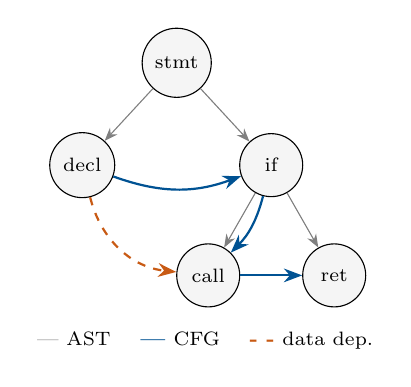
\begin{tikzpicture}[
          n/.style={draw, circle, minimum size=0.8cm, font=\scriptsize, fill=gray!8},
          ast/.style={-{Stealth}, gray},
          cfg/.style={-{Stealth}, thick, IITGBlue},
          ddg/.style={-{Stealth}, thick, hl, dashed}]
        \node[n] (a) at (0,0) {stmt};
        \node[n] (b) at (-1.2,-1.3) {decl};
        \node[n] (c) at (1.2,-1.3) {if};
        \node[n] (d) at (0.4,-2.7) {call};
        \node[n] (e) at (2.0,-2.7) {ret};
        \draw[ast] (a) -- (b);
        \draw[ast] (a) -- (c);
        \draw[ast] (c) -- (d);
        \draw[ast] (c) -- (e);
        \draw[cfg] (b) to[bend right=20] (c);
        \draw[cfg] (c) to[bend left=15] (d);
        \draw[cfg] (d) -- (e);
        \draw[ddg] (b) to[bend right=35] (d);
        \node[font=\scriptsize, align=left, anchor=north west] at (-1.9,-3.3)
          {\textcolor{gray}{---} AST \quad
           \textcolor{IITGBlue}{\textbf{---}} CFG \quad
           \textcolor{hl}{\textbf{- -}} data dep.};
      \end{tikzpicture}
    \end{column}
  \end{columns}
\end{frame}

% ----------------------------------------------------------------
\begin{frame}{Earlier Tools}
  \begin{columns}[T]
    \begin{column}{0.32\textwidth}
      \textbf{tree-sitter}
      \begin{itemize}
        \item Syntax tree only
      \end{itemize}
      \textcolor{badred}{\textbf{Drawbacks}}
      \begin{itemize}
        \item No names / types
        \item No CFG / data flow
        \item Calls matched by name
      \end{itemize}
    \end{column}
    \begin{column}{0.32\textwidth}
      \textbf{Joern}
      \begin{itemize}
        \item CPG platform
      \end{itemize}
      \textcolor{badred}{\textbf{Drawbacks}}
      \begin{itemize}
        \item Fuzzy parsing, no compile
        \item Types, overloads guessed
        \item Macros, headers only as parsed
      \end{itemize}
    \end{column}
    \begin{column}{0.32\textwidth}
      \textbf{ATLAS}
      \begin{itemize}
        \item AST + CFG + DFG
      \end{itemize}
      \textcolor{badred}{\textbf{Drawbacks}}
      \begin{itemize}
        \item Files merged into one unit
        \item Unknown types become wildcards
        \item No operator overloading, \code{goto}
      \end{itemize}
    \end{column}
  \end{columns}

  \vspace{1.2em}
  \begin{exampleblock}{}
    \centering
    None compile the code, so their CFG and DFG are \textbf{approximated}
  \end{exampleblock}
\end{frame}

% ----------------------------------------------------------------
\begin{frame}{Our Approach vs.\ Earlier Tools}
  \centering
  \small
  \renewcommand{\arraystretch}{1.3}
  \begin{tabular}{l c c c c}
    \toprule
    & \textbf{tree-sitter} & \textbf{Joern} & \textbf{ATLAS} & \textbf{Ours} \\
    \midrule
    Exact types      & \xmark & \pmark & \pmark & \cmark \\
    CFG              & \xmark & \pmark & \pmark & \cmark \\
    Data flow        & \xmark & \pmark & \pmark & \cmark \\
    Multiple TUs     & \xmark & \pmark & \pmark & \cmark \\
    No build needed  & \cmark & \cmark & \cmark & \xmark \\
    \bottomrule
  \end{tabular}

  \vspace{0.5em}
  \scriptsize \cmark\ exact \quad \pmark\ approximate \quad \xmark\ none
\end{frame}

% ================================================================
\section{Our Approach}
% ================================================================

% ----------------------------------------------------------------
\begin{frame}{System Pipeline}
  \centering
  \begin{tikzpicture}[
      box/.style={draw, rounded corners, align=center, font=\small,
                  minimum height=0.9cm, minimum width=2.2cm, fill=gray!8},
      key/.style={box, fill=hl!18, draw=hl},
      out/.style={box, fill=IITGBlue!10, draw=IITGBlue, minimum width=1.6cm},
      arr/.style={-{Stealth[length=2.3mm]}, thick}]
    \node[box] (src) {\code{.c} / \code{.cpp}\\(one per TU)};
    \node[key, right=0.5cm of src] (clang) {clang\\\code{-emit-cir}};
    \node[box, right=0.5cm of clang] (cir) {\code{.cir}\\text};
    \node[key, right=0.5cm of cir] (build) {Graph builder\\blocks, SSA};
    \node[key, below=0.9cm of build] (mem) {Memory model\\reaching defs};
    \node[key, left=0.5cm of mem] (link) {Linker\\TUs, calls, SCCs};
    \node[out, left=0.9cm of link, yshift=0.55cm] (kuzu) {K\`uzu DB};
    \node[out, left=0.9cm of link, yshift=-0.55cm] (json) {JSON / DOT};
    \draw[arr] (src) -- (clang);
    \draw[arr] (clang) -- (cir);
    \draw[arr] (cir) -- (build);
    \draw[arr] (build) -- (mem);
    \draw[arr] (mem) -- (link);
    \draw[arr] (link) -- (kuzu);
    \draw[arr] (link) -- (json);
  \end{tikzpicture}

  \vspace{1em}
  \begin{itemize}
    \item Uses the project's real build flags
    \item Pure-Python engine: no LLVM build needed to build the graph
    \item Output: \textbf{K\`uzu} graph database, queried with \textbf{Cypher}
  \end{itemize}
\end{frame}

% ----------------------------------------------------------------
\begin{frame}{One Whole-Program Graph, Three Levels}
  \centering
  \begin{tikzpicture}[
      lay/.style={draw, rounded corners, fill=#1, minimum height=0.85cm,
                  text width=12.6cm, align=left, anchor=north west,
                  font=\footnotesize, inner xsep=6pt},
      conn/.style={-{Stealth[length=1.8mm]}, thick, black!70},
      cl/.style={right, font=\tiny\ttfamily, black!70}]
    \newcommand{\lname}[1]{\makebox[2.35cm][l]{\small\textbf{#1}}}
    \newcommand{\rel}[1]{\;$\xrightarrow{\text{\tiny\ttfamily #1}}$\;}
    \newcommand{\props}[1]{\hfill{\color{black!55}\scriptsize #1}}
    \node[lay=IITGBlue!12] (m) at (0,0)
      {\lname{FUNCTION}Program $\to$ TranslationUnit $\to$ Function\rel{CALLS}Function
       \props{call graph}};
    \node[lay=okgreen!10] (s) at (0,-1.25)
      {\lname{BLOCK}BasicBlock\rel{CFG\_NEXT}BasicBlock
       \props{control flow}};
    \node[lay=hl!12] (u) at (0,-2.5)
      {\lname{OPERATION}Operation\rel{DEFINES / USES}Value\rel{FLOWS\_TO}Value
       \props{data flow}};
    \node[lay=gray!12] (b) at (0,-3.75)
      {\lname{BRIDGES}call\rel{INVOKES}callee;\; argument $\to$ parameter;\;
       return $\to$ call result};
    \draw[conn] (1.1,-0.85) -- node[cl]{HAS\_BLOCK} (1.1,-1.25);
    \draw[conn] (1.1,-2.10) -- node[cl]{CONTAINS\_OPERATION} (1.1,-2.5);
  \end{tikzpicture}

  \vspace{1em}
  \begin{itemize}
    \item All levels share the \textbf{same} node IDs: one query crosses levels
    \item 8 node types, 15 relationship types
  \end{itemize}
\end{frame}

% ----------------------------------------------------------------
\begin{frame}{Building the Function Level}
  \begin{columns}[c]
    \begin{column}{0.42\textwidth}
      \begin{itemize}
        \item Program, TUs, functions, globals
        \item \textbf{Linking} by mangled symbol
              \begin{itemize}
                \item \code{extern} decl linked to definition in another TU
                \item \code{static}: TU-scoped, never merged
              \end{itemize}
        \item \code{CALLS} edges (\code{isCrossTU})
        \item Function pointers resolved when traceable
        \item Recursion (Tarjan SCC), unreachable functions
      \end{itemize}
    \end{column}
    \begin{column}{0.56\textwidth}
      \centering
      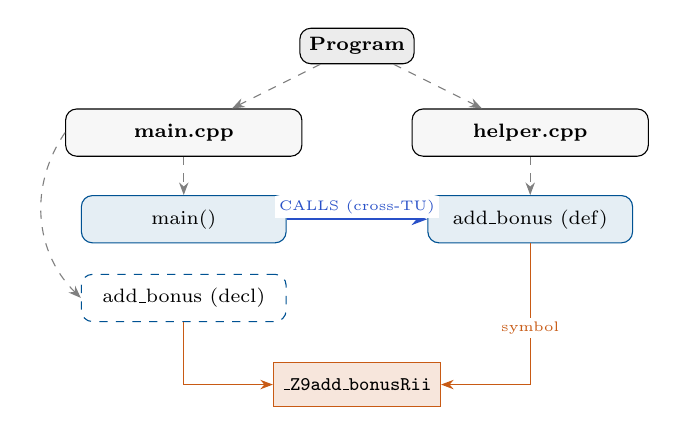
\begin{tikzpicture}[
          tu/.style={draw, rounded corners, fill=gray!6, font=\scriptsize\bfseries,
                     minimum width=3.0cm, minimum height=0.6cm},
          fn/.style={draw, rounded corners, fill=IITGBlue!10, draw=IITGBlue,
                     font=\scriptsize, align=center, minimum width=2.6cm, minimum height=0.6cm},
          dc/.style={fn, dashed, fill=white},
          sym/.style={draw, fill=hl!15, draw=hl, font=\scriptsize\ttfamily,
                      minimum height=0.55cm},
          cont/.style={-{Stealth[length=1.6mm]}, gray, dashed},
          call/.style={-{Stealth[length=2mm]}, thick, callblue},
          el/.style={font=\tiny, inner sep=1.5pt, fill=white}]
        \node[draw, rounded corners, fill=gray!15, font=\scriptsize\bfseries]
          (prog) at (2.2,0) {Program};
        \node[tu] (t1) at (0,-1.1) {main.cpp};
        \node[tu] (t2) at (4.4,-1.1) {helper.cpp};
        \node[fn] (main) at (0,-2.2) {main()};
        \node[dc] (decl) at (0,-3.2) {add\_bonus (decl)};
        \node[fn] (def)  at (4.4,-2.2) {add\_bonus (def)};
        \node[sym] (s) at (2.2,-4.3) {\_Z9add\_bonusRii};
        \draw[cont] (prog) -- (t1);
        \draw[cont] (prog) -- (t2);
        \draw[cont] (t1) -- (main);
        \draw[cont] (t1.west) to[bend right=40] (decl.west);
        \draw[cont] (t2) -- (def);
        \draw[-{Stealth[length=1.6mm]}, hl] (decl.south) |- (s.west);
        \draw[-{Stealth[length=1.6mm]}, hl] (def.south) |- node[el, pos=0.3]{symbol} (s.east);
        \draw[call] (main) -- node[el, above]{CALLS (cross-TU)} (def);
      \end{tikzpicture}
    \end{column}
  \end{columns}
\end{frame}

% ----------------------------------------------------------------
\begin{frame}{Building the Block Level}
  \begin{columns}[c]
    \begin{column}{0.42\textwidth}
      \begin{itemize}
        \item Structured regions lowered to \textbf{basic blocks}
              \begin{itemize}
                \item condition, body, join blocks
                \item for \code{if}, loops, \code{switch}, \code{?:}
              \end{itemize}
        \item \code{CFG\_NEXT} edges
              \begin{itemize}
                \item kind: true / false / case / exception
                \item \textbf{back edges} flagged (loops)
              \end{itemize}
        \item \code{break}, \code{continue}, \code{goto} linked to targets
        \item Exit blocks marked
        \item Each operation in exactly one block
      \end{itemize}
    \end{column}
    \begin{column}{0.56\textwidth}
      \centering
      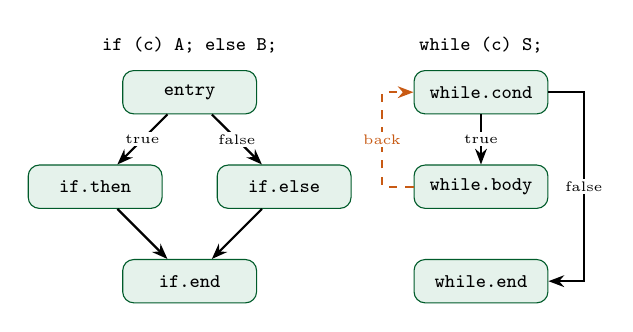
\begin{tikzpicture}[
          bb/.style={draw, rounded corners, fill=okgreen!10, draw=okgreen!70!black,
                     font=\scriptsize\ttfamily, minimum width=1.7cm, minimum height=0.55cm},
          e/.style={-{Stealth[length=2mm]}, thick},
          el/.style={font=\tiny, inner sep=1pt, fill=white}]
        % if / else
        \node[font=\scriptsize\bfseries] at (1.5,0.6) {\code{if (c) A; else B;}};
        \node[bb] (c)  at (1.5,0)    {entry};
        \node[bb] (t)  at (0.3,-1.2) {if.then};
        \node[bb] (f)  at (2.7,-1.2) {if.else};
        \node[bb] (j)  at (1.5,-2.4) {if.end};
        \draw[e] (c) -- node[el]{true} (t);
        \draw[e] (c) -- node[el]{false} (f);
        \draw[e] (t) -- (j);
        \draw[e] (f) -- (j);
        % while
        \node[font=\scriptsize\bfseries] at (5.2,0.6) {\code{while (c) S;}};
        \node[bb] (wc) at (5.2,0)    {while.cond};
        \node[bb] (wb) at (5.2,-1.2) {while.body};
        \node[bb] (we) at (5.2,-2.4) {while.end};
        \draw[e] (wc) -- node[el]{true} (wb);
        \draw[e] (wc.east) -- ++(0.45,0) |- node[el, pos=0.25]{false} (we.east);
        \draw[e, hl, dashed] (wb.west) -- ++(-0.4,0) |- node[el, pos=0.25, text=hl]{back} (wc.west);
      \end{tikzpicture}
    \end{column}
  \end{columns}
\end{frame}

% ----------------------------------------------------------------
\begin{frame}{Building the Operation Level}
  \begin{columns}[T]
    \begin{column}{0.48\textwidth}
      \textbf{Nodes and edges}
      \begin{itemize}
        \item Operation \code{-DEFINES/USES$\to$} Value
        \item Value \code{-FLOWS\_TO$\to$} Value, by kind:
      \end{itemize}
      \vspace{0.2em}
      \small
      \renewcommand{\arraystretch}{1.15}
      \begin{tabular}{@{\hspace{1.2em}}l l@{}}
        \toprule
        \code{def\_use} & operand $\to$ result \\
        \code{store\_to\_load} & through memory \\
        \code{call\_argument} & argument $\to$ parameter \\
        \code{call\_return} & return $\to$ call result \\
        \code{block\_arg}, \code{region\_yield} & between blocks / regions \\
        \bottomrule
      \end{tabular}
    \end{column}
    \begin{column}{0.48\textwidth}
      \textbf{Memory model}
      \begin{itemize}
        \item Abstract locations: locals, globals, pointer params, fields, elements
        \item \textbf{May-reaching definitions} over the CFG
              \begin{itemize}
                \item flow-sensitive, not path-sensitive
              \end{itemize}
        \item \textbf{Write summaries} for pointer / reference params
              \begin{itemize}
                \item replayed at each call site
              \end{itemize}
      \end{itemize}
    \end{column}
  \end{columns}
\end{frame}

% ================================================================
\section{Worked Example}
% ================================================================

% ----------------------------------------------------------------
\begin{frame}[fragile]{Example: A Side Effect Across Two TUs}
  \begin{columns}[T]
    \begin{column}{0.28\textwidth}
\begin{lstlisting}[language=C++, basicstyle=\ttfamily\footnotesize]
// api.h
#pragma once
void add_bonus(int &amount,
               int bonus);
\end{lstlisting}
    \end{column}
    \begin{column}{0.36\textwidth}
\begin{lstlisting}[language=C++, basicstyle=\ttfamily\footnotesize]
// main.cpp
#include "api.h"
int main() {
  int total = 10;
  add_bonus(total, 5);
  return total == 15 ? 0 : 1;
}
\end{lstlisting}
    \end{column}
    \begin{column}{0.33\textwidth}
\begin{lstlisting}[language=C++, basicstyle=\ttfamily\footnotesize]
// helper.cpp
#include "api.h"
void add_bonus(int &amount,
               int bonus) {
  if (bonus > 0) {
    amount = amount + bonus;
  }
}
\end{lstlisting}
    \end{column}
  \end{columns}

  \vspace{1.2em}
  \begin{itemize}
    \item \code{total} passed \textbf{by reference}; written in \textbf{another TU}
    \item Nothing at the call site shows the write
    \item Graph must link the helper's store to \code{main}'s later load of \code{total}
  \end{itemize}
\end{frame}

% ----------------------------------------------------------------
\begin{frame}{Example: Call Graph and CFG}
  \centering
  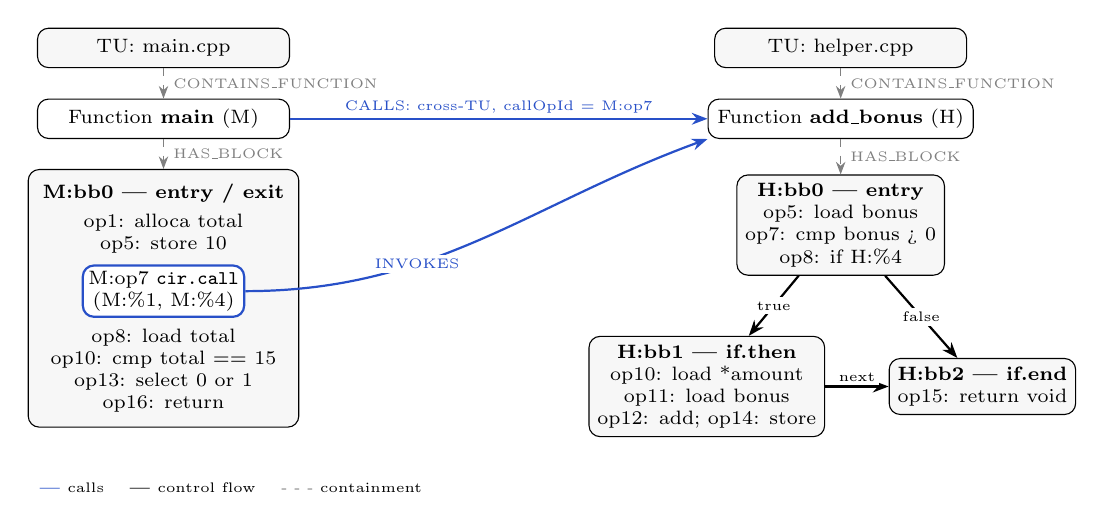
\begin{tikzpicture}[
      tu/.style={draw, rounded corners, fill=gray!6, font=\scriptsize,
                 minimum width=3.2cm, minimum height=0.5cm},
      fn/.style={draw, rounded corners, fill=white, font=\scriptsize,
                 minimum width=3.2cm, minimum height=0.5cm},
      bb/.style={draw, rounded corners, fill=gray!6, font=\scriptsize,
                 align=center, inner sep=3pt},
      op/.style={font=\scriptsize, align=center, inner sep=1pt},
      cont/.style={-{Stealth[length=1.6mm]}, gray, dashed},
      cl/.style={font=\tiny, gray, right},
      call/.style={-{Stealth[length=2mm]}, thick, callblue},
      cf/.style={-{Stealth[length=2mm]}, thick},
      el/.style={font=\tiny, inner sep=1.5pt, fill=white}]
    % ---- main.cpp
    \node[tu] (tum) at (0,0) {TU: main.cpp};
    \node[fn] (fm)  at (0,-0.9) {Function \textbf{main} (M)};
    \node[op, font=\scriptsize\bfseries] (mh) at (0,-1.85) {M:bb0 --- entry / exit};
    \node[op, below=0.05cm of mh] (m1) {op1: alloca total\\op5: store 10};
    \node[draw=callblue, thick, rounded corners, fill=white, font=\scriptsize,
          align=center, inner sep=2pt, below=0.1cm of m1] (mc)
          {M:op7 \code{cir.call}\\(M:\%1, M:\%4)};
    \node[op, below=0.1cm of mc] (m2) {op8: load total\\op10: cmp total == 15\\
                                      op13: select 0 or 1\\op16: return};
    \begin{scope}[on background layer]
      \node[bb, fit=(mh)(m1)(mc)(m2), inner sep=4pt] (mbb) {};
    \end{scope}
    \draw[cont] (tum) -- node[cl]{CONTAINS\_FUNCTION} (fm);
    \draw[cont] (fm) -- node[cl]{HAS\_BLOCK} (mbb.north);
    % ---- helper.cpp
    \node[tu] (tuh) at (8.6,0) {TU: helper.cpp};
    \node[fn] (fh)  at (8.6,-0.9) {Function \textbf{add\_bonus} (H)};
    \node[bb] (h0) at (8.6,-2.25) {\textbf{H:bb0 --- entry}\\op5: load bonus\\
                                   op7: cmp bonus > 0\\op8: if H:\%4};
    \node[bb] (h1) at (6.9,-4.3) {\textbf{H:bb1 --- if.then}\\op10: load *amount\\
                                  op11: load bonus\\op12: add; op14: store};
    \node[bb] (h2) at (10.4,-4.3) {\textbf{H:bb2 --- if.end}\\op15: return void};
    \draw[cont] (tuh) -- node[cl]{CONTAINS\_FUNCTION} (fh);
    \draw[cont] (fh) -- node[cl]{HAS\_BLOCK} (h0);
    \draw[cf] (h0) -- node[el]{true} (h1);
    \draw[cf] (h0) -- node[el]{false} (h2);
    \draw[cf] (h1) -- node[el, above]{next} (h2);
    % ---- calls
    \draw[call] (fm) -- node[el, above, text=callblue]{CALLS: cross-TU, callOpId = M:op7} (fh);
    \draw[call] (mc.east) to[out=0, in=200] node[el, pos=0.35, text=callblue]{INVOKES} (fh.south west);
    % legend
    \node[font=\tiny, anchor=north west, align=left] at (-1.7,-5.4)
      {\textcolor{callblue}{\textbf{---}} calls \quad
       \textbf{---} control flow \quad
       \textcolor{gray}{- - -} containment};
  \end{tikzpicture}
\end{frame}

% ----------------------------------------------------------------
\begin{frame}[fragile]{Example: Data Flow (\code{FLOWS\_TO})}
  \centering
  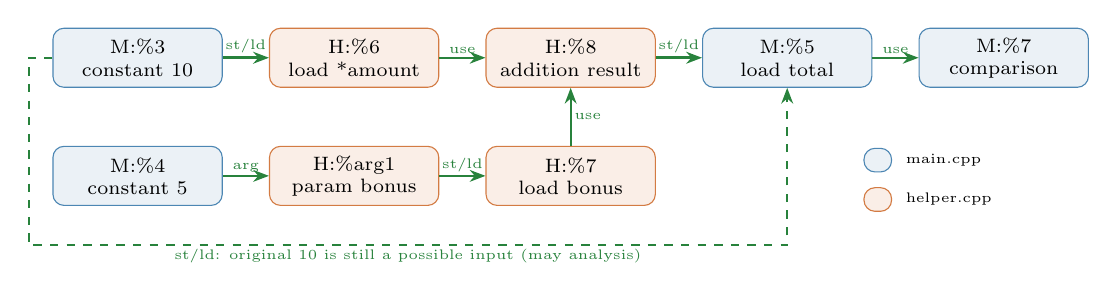
\begin{tikzpicture}[
      vm/.style={draw, rounded corners, fill=IITGBlue!8, draw=IITGBlue!70,
                 font=\scriptsize, align=center, minimum width=2.15cm, minimum height=0.75cm},
      vh/.style={vm, fill=hl!10, draw=hl!80},
      fl/.style={-{Stealth[length=2mm]}, thick, flowgreen},
      ip/.style={fl, very thick},
      el/.style={font=\tiny, inner sep=1pt, text=flowgreen, above}]
    % row 1
    \node[vm] (c10)  at (0,0)     {M:\%3\\constant 10};
    \node[vh] (ldA)  at (2.75,0)  {H:\%6\\load *amount};
    \node[vh] (add)  at (5.5,0)   {H:\%8\\addition result};
    \node[vm] (ldT)  at (8.25,0)  {M:\%5\\load total};
    \node[vm] (cmp)  at (11,0)    {M:\%7\\comparison};
    % row 2
    \node[vm] (c5)   at (0,-1.5)    {M:\%4\\constant 5};
    \node[vh] (pb)   at (2.75,-1.5) {H:\%arg1\\param bonus};
    \node[vh] (ldB)  at (5.5,-1.5)  {H:\%7\\load bonus};
    \draw[ip] (c10) -- node[el]{st/ld} (ldA);
    \draw[fl] (ldA) -- node[el]{use} (add);
    \draw[ip] (add) -- node[el]{st/ld} (ldT);
    \draw[fl] (ldT) -- node[el]{use} (cmp);
    \draw[fl] (c5)  -- node[el]{arg} (pb);
    \draw[fl] (pb)  -- node[el]{st/ld} (ldB);
    \draw[fl] (ldB) -- node[el, right]{use} (add);
    \draw[fl, dashed] (c10.west) -- ++(-0.3,0) |-
      node[el, below, pos=0.75]{st/ld: original 10 is still a possible input (may analysis)}
      ($(ldT.south)+(0,-2.0)$) -- (ldT.south);
    % legend
    \node[vm, minimum width=0.35cm, minimum height=0.3cm] (lgm) at (9.4,-1.3) {};
    \node[font=\tiny, right=0.05cm of lgm] {main.cpp};
    \node[vh, minimum width=0.35cm, minimum height=0.3cm] (lgh) at (9.4,-1.8) {};
    \node[font=\tiny, right=0.05cm of lgh] {helper.cpp};
  \end{tikzpicture}

  \vspace{0.6em}
  \begin{columns}[T]
    \begin{column}{0.52\textwidth}
\begin{lstlisting}[language=Cypher]
MATCH (s:Value)-[r:FLOWS_TO]->(v:Value)
WHERE r.kind = 'store_to_load'
  AND v.varName = 'total'
RETURN s.id, r.isInterprocedural
\end{lstlisting}
    \end{column}
    \begin{column}{0.44\textwidth}
      \small
      Returns both stores:
      \begin{itemize}
        \item initial \code{10} (local)
        \item helper's sum (\textbf{interprocedural})
      \end{itemize}
    \end{column}
  \end{columns}
\end{frame}

% ================================================================
\section{Case Study: Test Generation}
% ================================================================

% ----------------------------------------------------------------
\begin{frame}{Case Study: Problem Statement}
  \textbf{ICSE 2027 Industry Challenge 8}: project-specific test generation
  with validation intentions

  \vspace{0.8em}
  \begin{itemize}
    \item \textbf{Input}: project $P$, focal method $m$, natural-language intention $i$
    \item \textbf{Output}: a test that builds against $P$ and checks $i$
    \item \textbf{Targets} vs.\ source-browsing agents
          \begin{itemize}
            \item $\geq$\textbf{50\%} fewer tokens
            \item $\geq$\textbf{20\%} less time
          \end{itemize}
    \item \textbf{Repos}: libgit2, PostgreSQL, Qt Base, Binutils, U-Boot (up to 12.8k files)
    \item \textbf{Agents}: Codex, OpenHands (frontier model);
          OpenHands + private \textbf{Qwen3-Coder-30B}
  \end{itemize}
\end{frame}

% ----------------------------------------------------------------
\begin{frame}{Case Study: The Graph as Agent Context}
  \begin{columns}[c]
    \begin{column}{0.55\textwidth}
      \centering
      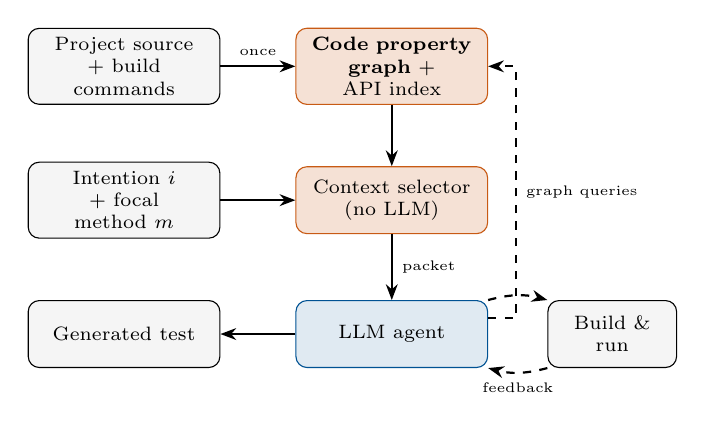
\begin{tikzpicture}[
          box/.style={draw, rounded corners, align=center, font=\scriptsize,
                      minimum height=0.85cm, fill=gray!8, text width=2.2cm},
          key/.style={box, fill=hl!18, draw=hl},
          llm/.style={box, fill=IITGBlue!12, draw=IITGBlue},
          arr/.style={-{Stealth[length=2mm]}, thick},
          fb/.style={-{Stealth[length=2mm]}, thick, dashed}]
        \node[box] (proj) at (0,0) {Project source\\+ build commands};
        \node[key] (graph) at (3.4,0) {\textbf{Code property}\\\textbf{graph} + API index};
        \node[box] (req) at (0,-1.7) {Intention $i$\\+ focal method $m$};
        \node[key] (sel) at (3.4,-1.7) {Context selector\\(no LLM)};
        \node[llm] (agent) at (3.4,-3.4) {LLM agent};
        \node[box] (test) at (0,-3.4) {Generated test};
        \node[box, text width=1.4cm] (build) at (6.2,-3.4) {Build \&\\run};
        \draw[arr] (proj) -- node[above, font=\tiny]{once} (graph);
        \draw[arr] (graph) -- (sel);
        \draw[arr] (req) -- (sel);
        \draw[arr] (sel) -- node[right, font=\tiny]{packet} (agent);
        \draw[arr] (agent) -- (test);
        \draw[fb] (agent.north east) to[bend left=15] (build.north west);
        \draw[fb] (build.south west) to[bend left=15] node[below, font=\tiny]{feedback} (agent.south east);
        \draw[fb] (agent.east) ++(0,0.2) -- ++(0.35,0) |- node[right, font=\tiny, pos=0.25]{graph queries} (graph.east);
      \end{tikzpicture}
    \end{column}
    \begin{column}{0.43\textwidth}
      \begin{itemize}
        \item \textbf{Packet} (9--32\,KB)
              \begin{itemize}
                \item focal declaration
                \item setup / cleanup APIs, types
              \end{itemize}
        \item \textbf{Graph queries as tools}
              \begin{itemize}
                \item functions, CFG, values, data flow
                \item expand only what is needed
              \end{itemize}
        \item \textbf{No source files read}
      \end{itemize}
    \end{column}
  \end{columns}
\end{frame}

% ----------------------------------------------------------------
\begin{frame}{Case Study: Results (23 tasks, source vs.\ graph)}
  \begin{columns}[T]
    \begin{column}{0.50\textwidth}
      \centering
      \textbf{Reductions, private Qwen model}\\[0.4em]
      \small
      \renewcommand{\arraystretch}{1.1}
      \begin{tabular}{l r r}
        \toprule
        Repository & Tokens & Time \\
        \midrule
        libgit2    & $-$77.4\% & $-$64.6\% \\
        PostgreSQL & $-$79.6\% & $-$55.4\% \\
        Qt Base    & $-$86.8\% & $-$78.5\% \\
        Binutils   & $-$76.1\% & $-$44.0\% \\
        U-Boot     & $-$57.5\% & $-$66.3\% \\
        \midrule
        \textbf{Pooled} & \textbf{$-$76.1\%} & \textbf{$-$62.1\%} \\
        \bottomrule
      \end{tabular}
    \end{column}
    \begin{column}{0.48\textwidth}
      \centering
      \textbf{Test quality, Qwen}\\[0.4em]
      \small
      \renewcommand{\arraystretch}{1.1}
      \begin{tabular}{l c c}
        \toprule
        & Source & Graph \\
        \midrule
        Full passes        & 10/23 & \textbf{17/23} \\
        Faults detected    & 25/59 & \textbf{46/59} \\
        Accepted on review & 10/23 & \textbf{19/23} \\
        Files read / task  & 2.7   & \textbf{0} \\
        \bottomrule
      \end{tabular}
    \end{column}
  \end{columns}

  \vspace{1em}
  \begin{itemize}
    \item Both targets met in \textbf{every} repository
    \item Frontier agents: $-$28--47\% tokens, $-$21--33\% time; all tests pass in both settings
  \end{itemize}
\end{frame}

% ================================================================
\section{Limitations and Future Work}
% ================================================================

% ----------------------------------------------------------------
\begin{frame}{Limitations and Future Work}
  \begin{columns}[T]
    \begin{column}{0.48\textwidth}
      \textbf{Limitations}
      \begin{itemize}
        \item No control-dependence edges
        \item No heap / points-to analysis
        \item No virtual-call edges
        \item Context-insensitive across calls
      \end{itemize}
    \end{column}
    \begin{column}{0.48\textwidth}
      \textbf{Future work}
      \begin{itemize}
        \item Control dependence (post-dominators), enabling \textbf{slicing}
        \item Stronger alias analysis
        \item Front end on MLIR APIs
        \item LLM-assisted code Q\&A over the graph
      \end{itemize}
    \end{column}
  \end{columns}
\end{frame}

% ----------------------------------------------------------------
\begin{frame}{Summary}
  \begin{itemize}
    \item \textbf{ClangIR}: compiler-accurate semantics with source-level structure
    \item \textbf{Our CPG}: whole-program, for C/C++
          \begin{itemize}
            \item function, block and operation levels on shared IDs
            \item cross-TU linking and data flow
            \item queryable with Cypher
          \end{itemize}
    \item \textbf{Case study}: as LLM context for test generation
          \begin{itemize}
            \item $-$76\% tokens, $-$62\% time (private model), better tests
          \end{itemize}
  \end{itemize}

  \vspace{1.5em}
  \centering
  {\Large \textbf{Thank you!}}\\[0.4em]
  Questions?
\end{frame}

\end{document}
